\documentclass[11pt]{article}
\usepackage[margin=1in]{geometry}
\usepackage{graphicx,booktabs,amsmath,amssymb}
\usepackage[T1]{fontenc}
\usepackage{listings,xcolor}
\lstdefinestyle{deck}{basicstyle=\ttfamily\footnotesize,columns=fullflexible,
  keepspaces=true,frame=single,rulecolor=\color{black!30},
  commentstyle=\color{blue!60!black}\itshape,escapechar=@}
\lstdefinestyle{py}{language=Python,basicstyle=\ttfamily\scriptsize,
  columns=fullflexible,keepspaces=true,frame=single,
  rulecolor=\color{black!30},commentstyle=\color{black!55}\itshape,
  keywordstyle=\color{blue!60!black},stringstyle=\color{green!40!black},
  breaklines=true}
\newcommand{\code}[1]{\texttt{#1}}
\title{Example 2: Transient response of a thick $(0/90/0)$ laminate ---\\
four-way benchmark anchored by the Khdeir--Reddy exact HSDT solution}
\author{OpenSG-RM dynamic validation suite (\code{examples/opensg-rm\_dynamic/ex2})}
\date{}
\begin{document}
\maketitle

\section{Why this case}
This is Example~2 of Nayak, Shenoi \& Moy, \emph{Composite Structures}
\textbf{64} (2004) 249--267, which is in turn the benchmark of Khdeir \&
Reddy, \emph{Composites Science and Technology} \textbf{34} (1989) 205--224
(Nayak's ref.~[11]): the one transient laminate problem for which an
\emph{analytical} solution of a shear-deformation plate theory exists in
closed form.  We run it \emph{first} because it separates the error sources
cleanly before the sandwich case (Example~5) is attempted:
(i)~the Khdeir--Reddy (KR) curve carries \emph{zero} discretization error
--- any difference between it and a converged FE of the same theory is a
bug; (ii)~the plate is deliberately \emph{thick} ($a/h=5$), so the
transverse-shear treatment of every 2-D theory is stressed to its limit;
(iii)~a 3-D solid model provides the physical truth, so each theory's
\emph{modeling} error is measured, not assumed.

\paragraph{How ``exact'' is the Khdeir--Reddy solution?}
It is exact \emph{within Reddy's third-order theory (HSDT)}: for a simply
supported cross-ply plate under a doubly sinusoidal load the Navier
expansion satisfies the HSDT field equations and boundary conditions
identically (single mode $m=n=1$), and the resulting 5-DOF ODE system is
integrated exactly in time (their state-space form; equivalently modal
superposition --- ``both procedures give the same result'').  It is
\textbf{not} 3-D elasticity: unlike Pagano's benchmark there is no exact
through-thickness solution here.  Consequently the \textbf{Abaqus 3-D
solid model is the benchmark} of this report and the KR solution is one of
the graded theories.

\section{Problem statement}
A simply supported (SS-1) \emph{square} cross-ply laminate:

\begin{center}\begin{tabular}{ll}\toprule
plate & $a=b=5h$, $h=0.1524$ m $\Rightarrow a=b=0.762$ m ($a/h=5$, thick)\\
layup & $(0/90/0)$, three equal-thickness plies of $h/3$ each\\
material & $E_1=172.369$ GPa, $E_2=6.895$ GPa ($E_1/E_2=25$)\\
 & $G_{12}=G_{13}=3.448$ GPa $(=0.5E_2)$, $G_{23}=1.379$ GPa $(=0.2E_2)$\\
 & $\nu_{12}=0.25$, $\rho=1603.03$ kg/m$^3$\\
load & $q(x,y,t)=q_0\,F(t)\sin(\pi x/a)\sin(\pi y/b)$, $q_0=68.9476$ MPa\\
window & 20 ms; shell increments fixed at $\Delta t=50\,\mu$s\\
reported & $w(a/2,b/2)/0.0254$ m (KR plot deflection in inches) and
$\bar\sigma_x=\sigma_x(a/2,b/2,h/2)/q_0$\\
\bottomrule\end{tabular}\end{center}

\paragraph{What ``transient analysis'' means here.}
A \emph{static} analysis asks only for the final equilibrium shape under a
load.  A \emph{transient} (time-history) analysis solves
$M\ddot u+Ku=f(t)$ through time: the load is applied suddenly, the plate's
\emph{inertia} resists, and the structure overshoots its static deflection
and then \emph{vibrates} about it.  For an undamped plate hit by a
suddenly applied constant pressure the center swings between $0$ and
$\approx2\times$ the static deflection, cycle after cycle --- which is why
the result of this analysis is a \emph{curve} $w(t)$, not a single number,
and why the peak of that curve (the design quantity) is about twice what a
static calculation would give.

\paragraph{The two pulses.}  $F(t)$ multiplies the spatial load:
\begin{equation}
F_{\rm step}(t)=\begin{cases}1,&0\le t\le t_1\\ 0,&t>t_1\end{cases}
\qquad
F_{\rm blast}(t)=e^{-\gamma t},
\qquad t_1=6\ {\rm ms},\ \ \gamma=330\ {\rm s}^{-1}.
\end{equation}
In words: the \textbf{step} pulse is a pressure switched on
\emph{instantly} at $t=0$, held constant for 6 ms, then switched off ---
like slamming a weight onto the plate and lifting it off again; after
removal the plate keeps vibrating freely on whatever motion it had.  The
\textbf{explosive blast} pulse is the classic idealization of a far-field
detonation: the over-pressure jumps to $q_0$ instantly and decays
exponentially (here to $1/e$ within 3 ms), so the plate receives a hard
initial kick whose push fades while the plate is still responding.  Both
start from rest (zero displacement and velocity).

\section{The four models}
\begin{enumerate}
\item \textbf{Abaqus 3-D solid (benchmark)}: $20\times20\times18$ C3D8I
  (6 incompatible-mode bricks per ply through the thickness), per-ply
  \code{*ORIENTATION}, SS-1 supports on the side faces, the double-sine
  pressure on the top face; automatic implicit-dynamic increments.
\item \textbf{OpenSG-RM} (\code{ex2\_RM\_*.inp}): a plain S4 mesh whose
  \emph{entire} constitutive input is the MSG-homogenized $8\times8$ ABDG
  of the through-thickness 1-D SG: the $6\times6$ enters as \code{*SHELL
  GENERAL SECTION}, the $2\times2$ shear block as \code{*TRANSVERSE SHEAR
  STIFFNESS} ($G_{11}=2.452\times10^{8}$, $G_{22}=2.658\times10^{8}$ N/m
  --- 30\,\% softer than the $5/6$-parallel FSDT value $3.50\times10^{8}$).
  No plies, no orientations, no shear-correction factor appear in the deck.
\item \textbf{Abaqus FSDT} (\code{ex2\_FSDT\_*.inp}): the conventional
  industry route --- \code{*SHELL SECTION, COMPOSITE} with the three plies;
  Abaqus assembles $A/B/D$ and its \emph{own} transverse-shear stiffness.
\item \textbf{Khdeir--Reddy exact HSDT}: evaluated by our
  \code{reddy\_hsdt\_navier.py} (Sec.~\ref{sec:kr}), \emph{not} by any
  finite-element run.
\end{enumerate}

\section{The Khdeir--Reddy reference, in brief}
\label{sec:kr}
The reference curve is the exact solution of Reddy's third-order plate
theory for this plate, as published by Khdeir \& Reddy (1989).  In plain
terms: for a simply supported cross-ply plate under the double-sine load,
the theory's response is carried by a \emph{single} vibration pattern
(one Navier mode), so the whole plate reduces to a small 5-unknown
oscillator system that can be integrated \emph{by formula} --- no mesh, no
time stepping, hence no numerical error \emph{of the theory's own
prediction}.  The implementation lives in
\code{ex2/reddy\_hsdt\_navier.py}; the reader who wants the equations can
read that file's comments --- they are not needed to use this report.

What matters practically is that the curve agrees with \textbf{Nayak's own
converged 9-node finite element} (his Table~3, $4\times4$ mesh,
$\Delta t=40\,\mu$s --- the values used everywhere below as ``their''
result), at his printed sample times ($w/0.0254$~m, step pulse):

\begin{center}\begin{tabular}{lccccc}\toprule
$t$ [ms] & 1.6 & 3.2 & 4.8 & 6.4 & 8.0\\\midrule
Nayak 9-node FE (Table 3) & 0.1870 & 0.6180 & 0.9983 & 0.4548 & $-$0.2191\\
exact HSDT (this suite)   & 0.2011 & 0.6540 & 1.0225 & 0.3737 & $-$0.3477\\
\bottomrule\end{tabular}\end{center}

\noindent 2--7\,\% at the pre-cut-off times, explained by his finite time
step and mesh (his own convergence study moves toward these values as
$\Delta t\!\downarrow$); the post-cut-off points are phase-sensitive
(Sec.~\ref{sec:results}).  His 4-node Table~2 is shear-locked and must
not be used as an anchor.

\section{The Abaqus decks, annotated}
\label{sec:decks}
Both shell decks are generated by \code{make\_abaqus\_ex2.py}; below every
keyword block of the \emph{OpenSG-RM} deck with its meaning
(\code{...}~marks elided repetitive data lines).

\begin{lstlisting}[style=deck]
*HEADING                                    @\color{blue!60!black}\itshape title line@
Nayak Ex.2 / Khdeir-Reddy 1989 (0/90/0) a=5h, OpenSG-RM 8x8 shell, step pulse
*NODE                                       @\color{blue!60!black}\itshape 21x21 nodes of the flat plate, z=0@
1, 0.00000000, 0.00000000, 0.0
...
*ELEMENT, TYPE=S4, ELSET=EALL               @\color{blue!60!black}\itshape 20x20 4-node shells@
1, 1, 2, 23, 22
...
*NSET, NSET=NCEN                            @\color{blue!60!black}\itshape the center node (a/2,b/2): w history@
221
*ELSET, ELSET=PATCHC                        @\color{blue!60!black}\itshape 2x2-element patch at the center:@
190, 191, 210, 211                          @\color{blue!60!black}\itshape resultants for the stress recovery@
*NSET, NSET=NX0 ... NXA ... NY0 ... NYB     @\color{blue!60!black}\itshape the four edge node rows@
*NSET, NSET=NALL, GENERATE                  @\color{blue!60!black}\itshape all nodes (drilling constraint)@
1, 441, 1
*SHELL GENERAL SECTION, ELSET=EALL, DENSITY=244.302
                                            @\color{blue!60!black}\itshape THE OpenSG-RM INPUT: the MSG 6x6@
1.790800e+10, 2.633600e+08, 9.480600e+09, ... @\color{blue!60!black}\itshape (upper triangle, 21 numbers)@
                                            @\color{blue!60!black}\itshape DENSITY = rho*h [kg/m2]@
*TRANSVERSE SHEAR STIFFNESS                 @\color{blue!60!black}\itshape the MSG 2x2 shear block G@
2.452400e+08, 2.657700e+08, -9.854700e-05   @\color{blue!60!black}\itshape K11, K22, K12@
*BOUNDARY                                   @\color{blue!60!black}\itshape SS-1 simple supports:@
NX0, 2, 3                                   @\color{blue!60!black}\itshape x-edges: v = w = 0@
NXA, 2, 3
NY0, 1, 1                                   @\color{blue!60!black}\itshape y-edges: u = 0 ...@
NYB, 1, 1
NY0, 3, 3                                   @\color{blue!60!black}\itshape ... and w = 0@
NYB, 3, 3
NALL, 6, 6                                  @\color{blue!60!black}\itshape drilling dof fixed (flat plate)@
*AMPLITUDE, NAME=FT                         @\color{blue!60!black}\itshape F(t): 1 up to t1=6ms, then 0@
0., 1., 0.006, 1., 0.006001, 0., 0.02, 0.   @\color{blue!60!black}\itshape (blast deck: $e^{-330t}$ tabulated)@
*STEP, NAME=PULSE, INC=800                  @\color{blue!60!black}\itshape implicit dynamics:@
*DYNAMIC
5e-05, 0.02, 5e-09, 5e-05                   @\color{blue!60!black}\itshape dt=50us, T=20ms, max inc=50us@
*DLOAD, AMPLITUDE=FT                        @\color{blue!60!black}\itshape the double-sine pressure, value@
1, P, 4.238810e+05                          @\color{blue!60!black}\itshape q0 sin sin at each element center@
...
*NODE PRINT, NSET=NCEN, FREQUENCY=1         @\color{blue!60!black}\itshape center U every increment@
U
*EL PRINT, ELSET=PATCHC, FREQUENCY=1        @\color{blue!60!black}\itshape patch resultants SF/SM + COORD@
SF, SM
*EL PRINT, ELSET=PATCHC, FREQUENCY=1
COORD
*END STEP
\end{lstlisting}

The \emph{conventional FSDT} deck is identical in mesh, sets, BCs, load and
step; only the section block differs --- Abaqus receives the \emph{plies}
and builds its own law:

\begin{lstlisting}[style=deck]
*MATERIAL, NAME=GE25                        @\color{blue!60!black}\itshape one lamina material@
*ELASTIC, TYPE=LAMINA                       @\color{blue!60!black}\itshape E1, E2, nu12, G12, G13, G23@
1.723690e+11, 6.895000e+09, 0.25, 3.448000e+09, 3.448000e+09, 1.379000e+09
*DENSITY
1603.03,
*SHELL SECTION, ELSET=EALL, COMPOSITE       @\color{blue!60!black}\itshape the 3 plies: thickness,@
0.0508, 3, GE25, 0                          @\color{blue!60!black}\itshape integration points, material,@
0.0508, 3, GE25, 90                         @\color{blue!60!black}\itshape ply angle -- Abaqus computes@
0.0508, 3, GE25, 0                          @\color{blue!60!black}\itshape A/B/D + its own shear stiffness@
\end{lstlisting}

\section{Results}
\label{sec:results}
\begin{figure}[h!]\centering
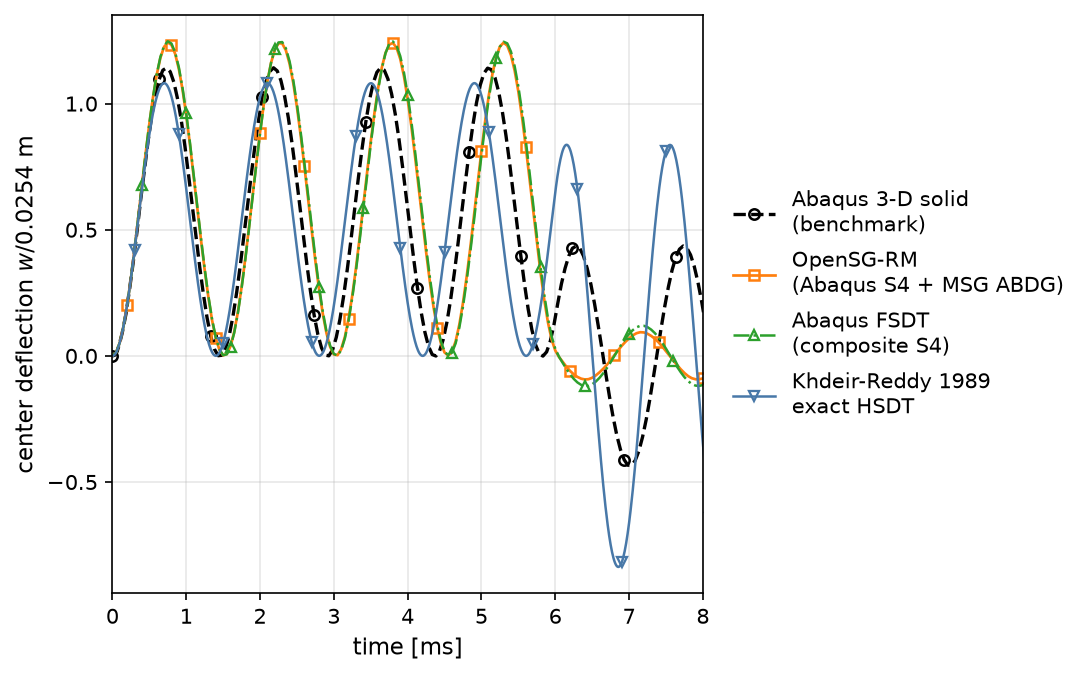
\includegraphics[width=.75\textwidth]{ex2_w_history_step.png}
\caption{Center deflection, step pulse (cut off at $t_1=6$ ms), four-way.}
\end{figure}
\begin{figure}[h!]\centering
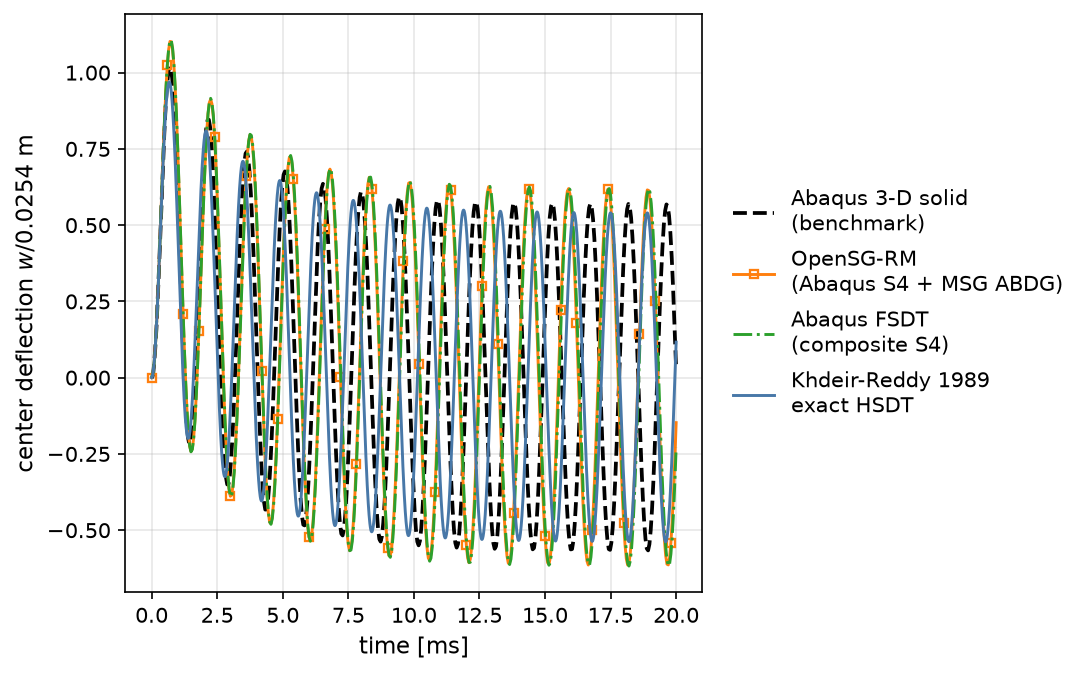
\includegraphics[width=.75\textwidth]{ex2_w_history_blast.png}
\caption{Center deflection, blast pulse $e^{-330t}$, four-way.}
\end{figure}
\begin{figure}[h!]\centering
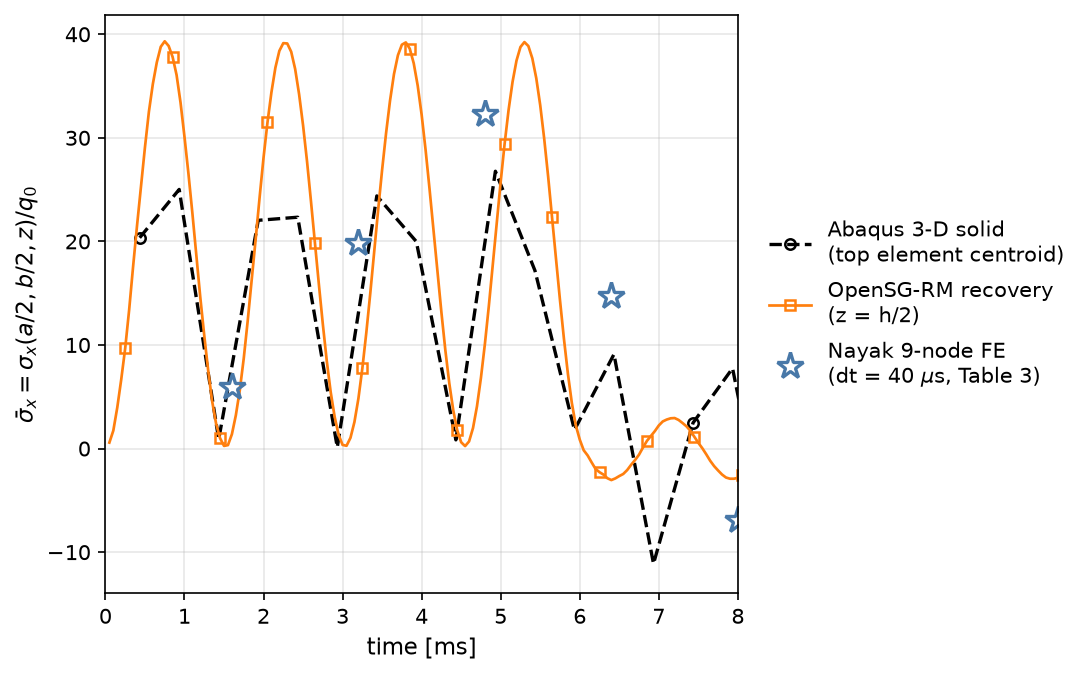
\includegraphics[width=.75\textwidth]{ex2_sx_history_step.png}
\caption{Top-surface normal stress $\bar\sigma_x$ at the center, step
pulse: solid (element centroid) vs.\ the OpenSG-RM recovery and the exact
HSDT at $z=h/2$.}
\end{figure}

\begin{center}\begin{tabular}{lcccc}\toprule
 & \multicolumn{2}{c}{step} & \multicolumn{2}{c}{blast}\\
model & peak $w/0.0254$ & \%~vs solid & peak $w/0.0254$ & \%~vs solid\\
\midrule
Abaqus 3-D solid (benchmark) & 1.1420 & --- & 1.0202 & ---\\
OpenSG-RM (S4 + MSG ABDG) & 1.2423 & $+8.8$ & 1.1023 & $+8.1$\\
Abaqus FSDT (composite S4) & 1.2470 & $+9.2$ & 1.1060 & $+8.4$\\
Khdeir--Reddy exact HSDT & 1.0810 & $-5.3$ & 0.9687 & $-5.1$\\
\bottomrule\end{tabular}\end{center}

\paragraph{Discussion.}
(i)~At $a/h=5$ \emph{every} plate theory carries several-percent error:
the HSDT under-predicts the peak by $\sim$5\,\%, the first-order theories
over-predict by 8--9\,\% --- only the 3-D solid arbitrates.
(ii)~\textbf{OpenSG-RM and the conventional Abaqus FSDT nearly coincide
here} (0.4 points apart): on an ordinary laminate the MSG shear block and
Abaqus's built-in composite shear treatment produce almost the same
section law.  The dramatic split between them is \emph{soft-core sandwich}
physics --- see the Example-5 report.
(iii)~The response oscillates with $T\approx1.4$ ms ($f_1=714$ Hz for the
HSDT); a few percent frequency difference de-phases the theories within
two cycles, so \emph{point-in-time} samples (Nayak's anchor times) are
meaningful only for same-theory comparisons; peaks, periods and the
overlaid histories are the valid cross-theory metrics.

\end{document}
